\documentclass[12pt]{article}

\usepackage[utf8]{inputenc}

\usepackage[dvipsnames]{xcolor}

\usepackage{array}
\newcolumntype{L}{>{\centering\arraybackslash}m{3cm}}

\usepackage{algorithm}
\usepackage{algpseudocode}
\usepackage{caption}

\usepackage{graphicx}
\usepackage{csquotes}

\renewcommand{\bibname}{References}


\title{Mathematical Optimization\\Final Project Report}

\author{Shayan Amani}

\date{\today}

\begin{document}
\maketitle

\section{Introduction}
Among available optimization algorithms, group of gradient descent have shown better performance in case of large data sets. This project is to compare these set of algorithms with a focus on understanding the approach of each.

\section{Motivation}
Advanced and popular differentiable programming frameworks are using gradient descent optimization variations at the core level. By exploring the documentation of these frameworks, it is visible that a specific set of the algorithms are in common. Understanding and getting a hands-on experience in implementation of these algorithms was the key factor to select this topic as my final project.

\section{Algorithms}
Gradient descent as an optimization technique includes three variations:
\begin{itemize}
    \item batch gradient descent,
    \item stochastic gradient descent, and 
    \item mini-batch gradient descent.
\end{itemize}
The examined algorithms are as follows:
\begin{itemize}
    \item Momentum \cite{NQianOnAlgorithms}
    \item Nesterov Accelerated Gradient \cite{NESTEROV1983AO1/k2}
    \item AdaGrad \cite{DuchiAdaptiveOptimization}
    \item AdaDelta \cite{Zeiler2012ADADELTA:Method}
    \item RMSprop \cite{HintonNeuralDescent}
    \item Adam \cite{KingmaAdam:Optimization}
    \item NAdam \cite{Dozat2016IncorporatingAdam}
\end{itemize}

\section{Implementation}
I have implemented the algorithm in python using numpy package. My idea is mimicking a set of neural network layers by only incorporating activation functions. The functions such as log, tanh, elu are considered here to test out the algorithms. MNIST dataset is used to calculate error in learning (cost function) by sequentially calculating functions value for each image of the dataset and plugging them into the algorithms' update equation.

\section{Results}
As figure \ref{fig:algorithms_cost_function} shows, the cost (error) of learning during 100 epochs varies by using a differnet algorithm. AdaDelta went to the no-return point and indicates \textit{no free lunch theorem} for optimization.
\begin{figure}
    \centering
    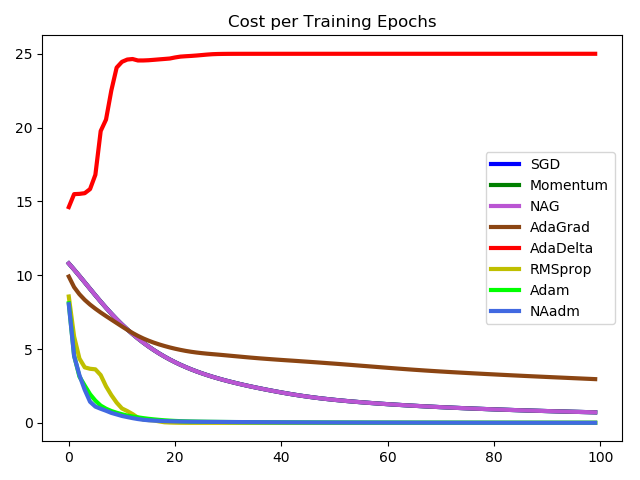
\includegraphics[width=1\columnwidth]{presentation/MathOpt-proj/myplot.png}
    \caption{Minimizing the error function in learning for 100 trials calculated using different algorithms.}
    \label{fig:algorithms_cost_function}
\end{figure}


\bibliographystyle{plain}
\bibliography{library}


\end{document}